% !TEX encoding = Windows Cyrillic
\documentclass[a4paper,12pt]{article}
\usepackage[mag=990]{newlistok}
\usepackage{tikz}
\usetikzlibrary{calc}

\УвеличитьШирину{1.4cm}
\УвеличитьВысоту{2.3cm}



\Заголовок{Гауссовы целые числа}
\НомерЛистка{42}
\renewcommand{\spacer}{\vspace{1.2pt}}
\ДатаЛистка{11.12.2019--25.12.2019}
\Оценки{22/18/14}

\begin{document}
	\СоздатьЗаголовок
	
	{\footnotesize В этом листке мы перенесём понятия делимости, общих делителей, разложения на простые сомножители на <<целые комплексные числа>>.}
	
	\опр Числа вида $a+bi$, где $a,b \in \mathbb{Z}$, называются \emph{гауссовыми целыми числами} или просто \emph{гауссовыми числами}. Множество всех гауссовых чисел обозначается $\mathbb{Z}[\sqrt{-1}]$ или $\Z[i]$. Легко видеть, что сумма и произведение гауссовых чисел -- снова гауссовы. Как обычно, скажем, что гауссово число $x$ {\em делит} гауссово число $y$, если существует такое гауссово $z$, что $y=xz$.
	
	Если $z = a+bi \neq 0$ --- гауссово число, то его \it{норма} $N(z) = |z|^2 = a^2+b^2$ --- натуральное число. Делимость гауссовых чисел связана с нормой, как показывает следующее утверждение.
	\копр 
	\пзадача  Докажите, что для всех $z \in \Z[i]$
	\пункт $z$ делит $N(z)$;
	\пункт если $x$ делит $y$, то $N(x)$ делит $N(y)$.
	\кзадача
	
	\задача Для следующих пар чисел выясните, делится ли какое-либо из них на другое, и найдите частное:
	$1+i$ и $8$; $2+i$ и $3+i$; $4-3i$ и $3+4i$.
	\кзадача
	
	\задача Докажите, что для гауссовых чисел $x$ и $y$ следующие свойства эквивалентны:
	(1) Множество делителей $x$ совпадает с множеством делителей $y$;	
	(2) $x$ делит $y$ и $y$ делит $x$; 
	(3) $x=ry$, где $N(r)=1$. 
	\кзадача
	
	\пзадача \пункт Гауссово число $x$ называется {\em обратимым}, если оно делит $1$. Докажите, что обратимые числа в точности числа с нормой 1.
	\пункт Найдите все обратимые гауссовы числа.
	\кзадача 
	
	{\footnotesize Как видно из задач 3 и 4, в гауссовых числах делимость <<не различает>> числа, получающиеся друг из друга умножением на обратимые. Такие числа называются {\it ассоциированными}. У ассоциированных чисел одинаковые делители и делимые. Как следствие, все свойства делимости (простота, обратимость, разложимость) одинаковы для ассоциированных чисел, а разложение на простые и наибольший общий делитель определены с точностью до ассоциированности.}
	
	\опр Гауссово необратимое число $x \neq 0$ называется {\em простым}, если для любого разложения $x=yz$ какое-то из чисел $y,z$ обратимо.
	 \копр
	\задача  Являются ли простыми следующие гауссовы числа: $-i$, $2$, $3$, $1+i$, $2+i$, $1+2i$? 
	\кзадача
	\задача Докажите, что гауссово число с простой нормой является простым. \кзадача
	\пзадача Докажите, что простые натуральные числа разбиваются на два непересекающиеся множества: простые гауссовы числа и числа, которые являются нормой простых гауссовых чисел.
	\кзадача 
	\задача \пункт Простое натуральное число $p$ является нормой гауссового числа тогда и только тогда, когда $p = a^2+b^2$ для натуральных $a,b$. \пункт 
	 Какие простые числа $p \leq 29$ являются простыми гауссовыми?
	 	\УстановитьГраницы{0cm}{10cm}
	  \пункт Сформулируйте гипотезу об этих числах в общем виде и докажите её (Указание: используйте задачу  14 из листка 23).
	\кзадача

	\задача Отметьте на картинке справа обратимые и простые числа. Для всех остальных найдите разложение в произведение простых. 
	\кзадача
	\задача \label{div} \пункт Нарисуйте на картинке справа все гауссовы числа, кратные $1+2i$. 
	\пункт  Докажите, что для любых гауссовых чисел $x,y$, $y \neq 0$ найдутся такие гауссовы  $q,r$, что $x=qy+r$ и $|r|<|y|$.
	
	\ВосстановитьГраницы
	\vspace{-5.5cm}
	\УстановитьГраницы{9cm}{0cm}
	{\hsize 4.1truecm
       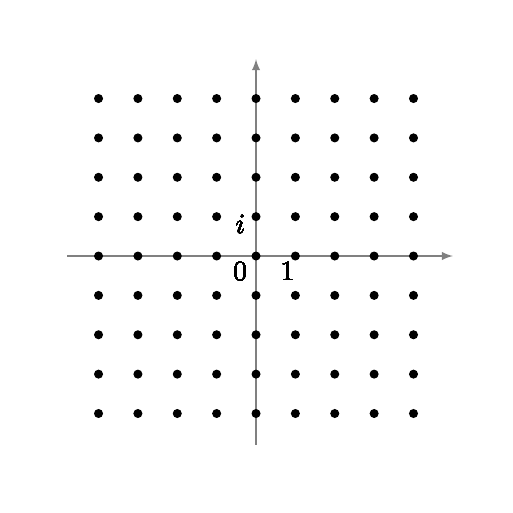
\begin{tikzpicture}
 %\Z[i]
    \coordinate (Origin)   at (0,0);
    \coordinate (XAxisMin) at (-2.4,0);
    \coordinate (XAxisMax) at (2.5,0);
    \coordinate (YAxisMin) at (0,-2.4);
    \coordinate (YAxisMax) at (0,2.5);
    \draw [thin, gray,-latex] (XAxisMin) -- (XAxisMax);% Draw x axis
    \draw [thin, gray,-latex] (YAxisMin) -- (YAxisMax);% Draw y axis
    \clip (-2.9,-2.9) rectangle (2.9cm,2.9cm); % Clips the picture...
    \coordinate (Bone) at (0,0.5);
    \coordinate (Btwo) at (0.5,0);
     \foreach \x in {-4,-3,...,4}{% Two indices running over each
      \foreach \y in {-4,-3,...,4}{% node on the grid we have drawn
        \node[draw,circle,inner sep=1pt,fill] at (\x/2,\y/2) {};
            % Places a dot at those points
         \node (n1) at (-0.2,-0.2) {$0$};
         \node (n2) at (0.4,-0.2) {$1$};
         \node (n3) at (-0.2,0.4) {$i$};
      }}
\end{tikzpicture}}
\hspace{-1cm}
	{\hsize 4.1truecm
       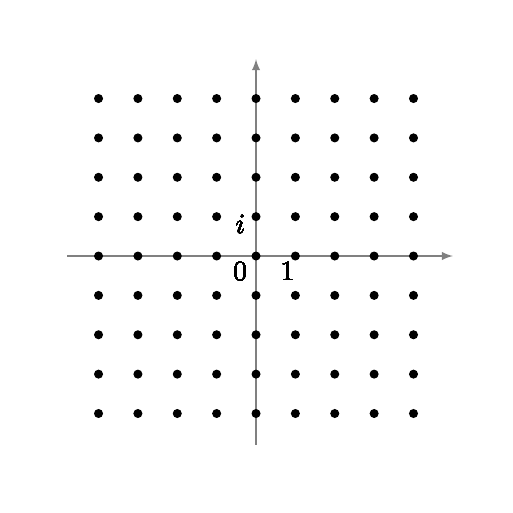
\begin{tikzpicture}
 %\Z[i]
    \coordinate (Origin)   at (0,0);
    \coordinate (XAxisMin) at (-2.4,0);
    \coordinate (XAxisMax) at (2.5,0);
    \coordinate (YAxisMin) at (0,-2.4);
    \coordinate (YAxisMax) at (0,2.5);
    \draw [thin, gray,-latex] (XAxisMin) -- (XAxisMax);% Draw x axis
    \draw [thin, gray,-latex] (YAxisMin) -- (YAxisMax);% Draw y axis
    \clip (-2.9,-2.9) rectangle (2.9cm,2.9cm); % Clips the picture...
    \coordinate (Bone) at (0,0.5);
    \coordinate (Btwo) at (0.5,0);
     \foreach \x in {-4,-3,...,4}{% Two indices running over each
      \foreach \y in {-4,-3,...,4}{% node on the grid we have drawn
        \node[draw,circle,inner sep=1pt,fill] at (\x/2,\y/2) {};
            % Places a dot at those points
         \node (n1) at (-0.2,-0.2) {$0$};
         \node (n2) at (0.4,-0.2) {$1$};
         \node (n3) at (-0.2,0.4) {$i$};
      }}
\end{tikzpicture}}

		\ВосстановитьГраницы
		\vspace{-0.4cm}
 \пункт Единственны ли такие $q,r$? Если нет, то сколько их может быть?
	\кзадача
	\задача Определите наибольший общий делитель двух гауссовых чисел, докажите, что он существует и представляется в виде их линейной комбинации (коэффициенты --- гауссовы).
	\кзадача
	\задача Найдите наибольший общий делитель чисел \пункт $7-i$ и $-4+7i$; \пункт $5+3i$ и $6-4i$.
	\кзадача
	
	\опр Гауссовы числа $x,y$ называются взаимно простыми, если их наибольший общий делитель обратим. \копр
	
	\пзадача  \пункт Верно ли, что целые числа $a$ и $b$ взаимно просты (как целые), если они взаимно просты как гауссовы? \пункт Верно ли обратное? \пункт Верно ли, что $x,y\in \Z[i]$ ---  гауссовы взаимно простые числа, если $N(x)$ и $N(y)$ --- взаимно просты (как натуральные)? \пункт Верно ли обратное?
	\кзадача
	\пзадача Докажите, что если гауссово простое делит произведение $xy$, то оно делит либо $x$, либо $y$.
	\кзадача
	\задача Сформулируйте и докажите основную теорему арифметики для гауссовых чисел.
	\кзадача
	\vspace{-0.2cm}
	\ЛичныйКондуит{0mm}{5mm}
	\end{document}
	
	\задача Решите в целых числах уравнение $y^3=x^2+1$.
	\кзадача
	\задача \пункт Докажите, что ни при каком $n$ число $(3+4i)^n$ не является вещественным.\\ \пункт Докажите, что угол $\arctg{3/4}$ не выражается рациональным числом градусов.\\ \спункт Найдите все такие натуральные $k$, что $\cos{\pi/k}$ и $\sin{\pi/k}$ рациональны.
	\кзадача
	\задача Докажите, что если два числа представимы в виде $a^2+db^2$ (где $d$ --- фиксированное натуральное число), то и их произведение представимо в таком виде.
	\кзадача
	\задача \пункт Дайте определение $\mathbb{Z}[\sqrt{-n}]$. \пункт Найдите все обратимые числа в $\mathbb{Z}[\sqrt{-n}]$. \пункт Верно ли утверждение задачи \ref{div}б) для $\mathbb{Z}[\sqrt{-n}]$? \пункт Однозначно ли разложение на множители в $\mathbb{Z}[\sqrt{-n}]$?
	\кзадача
	\задача \label{r} \пункт Обозначим через $r(n)$ количество решений уравнения $a^2+b^2=n$ в натуральных числах. Докажите, что если $m,n$ взаимно просты, то $r(mn)=r(m)r(n)$. \спункт Обозначим через $r_d(n)$ количество решений уравнения $a^2+db^2=n$ в целых числах. Верно ли предыдущее утверждение при $d>1$?
	\кзадача
	\задача Докажите, что число $1 000 009 = 235^2+972^2$ составное.
	\кзадача
	\сзадача \пункт Как посчитать $r(n)$ из задачи \ref{r}? \пункт Для каких натуральных $k$ существует окружность, на которой лежит ровно $k$ точек с целыми координатами?
	\кзадача

\ЛичныйКондуит{0mm}{5mm}
% \GenXMLW

\end{document}

%	\опр Функция $f: \mathbb{N} \to \mathbb{C}$ называется \emph{мультипликативной}, если для любых взаимно простых чисел $m,n$ имеется равенство $f(mn)=f(m)f(n)$. Важный для дальнейшего пример мультипликативной функции доставляет функция $\chi$, заданная по правилу $\chi(1)=1, \chi(2)=0,\chi(3)=-1, \chi(4)=0$, $\chi(4k+r)=\chi(r)$.
%	\копр
%	\задача Рассмотрим функцию $\rho(n) = \sum_{d|n} \chi(d)$. \пункт Докажите, что $\rho$ мультипликативна. \пункт Докажите, что $\rho(p^k)=r(p^k)$ (функция $r$ определяется в задаче \ref{r}) для всех простых $p$ и натуральных $k$, и тем самым эти две функции равны.
%	\кзадача
%	\задача Введём функцию $R(n) = \sum_{i=1}^n r(i)$, равную числу решений неравенства $a^2+b^2 \leqslant n$ в натуральных числах. \пункт Докажите, что $R(n)=\sum_{i=1}^n [\frac{n}{i}] \chi(i)$. \пункт Докажите, что $\lim\limits_{n \to \infty} \frac{R(n)}{n^2}=\frac{\pi}{4}$. \пункт Докажите формулу $\frac{\pi}{4}=1-\frac{1}{3}+\frac{1}{5}-\frac{1}{7}+\frac{1}{9}-\ldots$.
%	\кзадача
%	\задача \emph{Дзета-функция Римана} определяется равенством $\zeta(s) = \sum_{i=1}^{\infty} \frac{1}{i^s}$. \emph{$L$-функция Дирихле} определяется равенством $L(\chi,s)=\sum_{i=1}^{\infty} \frac{\chi(i)}{i^s}$. \пункт Докажите, что дзета-функция Римана равна эйлерову произведению $\prod_p (\frac{1}{1-1/p^s})$ и докажите аналогичную формулу для $L$-функции.  Следовательно, $\zeta(s)L(\chi,s)= \\ \big( \prod_{p=4k+1} (\frac{1}{1-1/p^s}) \big) \cdot \prod_{p=4k+3} (\frac{1}{1-1/p^{2s}})$. \пункт Докажите, что второе произведение имеет конечный ненулевой предел при $s \to 1$. Так как $L(\chi,1) \neq 0$, первое произведение не может иметь конечного предела при $s \to 1$. Следовательно, простых чисел вида $4k+1$ бесконечно много. \пункт Используя функции $\chi_0(n)$, равную $1$ при нечётных $n$, и $0$ иначе, и $L(\chi_0,s)=\sum_{i=1}^{\infty} \frac{\chi_0(i)}{i^s}$, докажите, что и произведение $\prod_{p=4k+3} (\frac{1}{1-1/p^s})$ не имеет конечного предела при $s \to 1$.
%	\кзадача
%	Петер Густав Лежён Дирихле в 1837 году доказал, что если $n,r$ взаимно просты, то найдётся бесконечно много простых чисел вида $kn+r$. Мы разобрали частный случай этого доказательства при $n=4$. Доказательство Дирихле использует обобщение рассмотренных нами результатов на случай области чисел вида $a_0+a_1\zeta+\ldots+a_{n-1}\zeta^{n-1}$, где $a_i \in \mathbb{Z}$, а $\zeta$ -- примитивный корень степени $n$ из $1$.
	
	
